\section{Portable two-speed residual experiment}
\label{sec:real-torque}
The fixture \texttt{psm\_dual\_system\_multirpm} contains 218 operating
points: 109 each at requested 1000 and 3000 rpm, with a 70-$^\circ$C rotor
temperature reference and $p=4$. Flux reconstruction uses measured mean
electrical speed; requested speed only groups comparable conditions. Measured
and requested quantities are not interchanged.

\subsection{Configuration qualification precedes residual interpretation}
Selector 1 represents two amplitude-invariant three-phase systems. With equal
represented system currents, total electromagnetic torque is
\begin{equation}
 M_{\mathrm{total}}=2\left[\frac32p(\psid\iq-\psiq\id)\right],
 \qquad \kt=3p=12.
 \label{eq:dual-system-torque}
\end{equation}
The earlier single-system factor $3p/2=6$ omitted half the represented total;
using the recorded configuration reduces the combined uncentered discrepancy
RMS from 19.71 to \SI{1.21}{\newton\metre}. This is a necessary configuration
diagnosis, not a fitted gain or the contribution claimed by this paper.

The CAN channel is transported numerically without a calibration certificate,
known shaft location, gear ratio or loss map. Its comparison with model torque
is conditional. No torque outlier deletion is applied, and the small-current
threshold is used only for normalized legacy diagnostics, not for fitting the
global residual.

\subsection{Offset, structure and a common correction}
With $r_M=M_{\mathrm{CAN}}-M_{\mathrm{theo}}$, the 1000-rpm group has bias
$-0.876$ Nm, uncentered RMS $0.958$ Nm and centered RMS $0.386$ Nm. At
3000 rpm these values are $-1.331$, $1.427$ and $0.515$ Nm. Thus much of the
uncentered discrepancy is an admissible group offset, but centering does not
remove all spatial variation.

A quadratic low-complexity residual surface reduces five-fold spatial
cross-validation RMS to $0.334$ Nm at 1000 rpm, compared with the constant
model's $0.386$ Nm. At 3000 rpm it gives $0.515$ versus $0.515$ Nm. The first
slice therefore contains reproducible slow structure; evidence for that model
extension is weak in the second. This diagnostic does not decide whether the
structure comes from flux, losses, voltage reconstruction or torque sensing.

Fit one co-energy correction shared by both speeds and a separate $c_g$ per
speed, using fixed $\lambda=10$. Centered residual RMS becomes $0.317$ Nm at
1000 rpm and $0.458$ Nm at 3000 rpm, with a $0.728$ mWb RMS flux change.
These are in-sample consistency improvements and cannot validate true flux.

\begin{figure}[htbp]
 \centering
 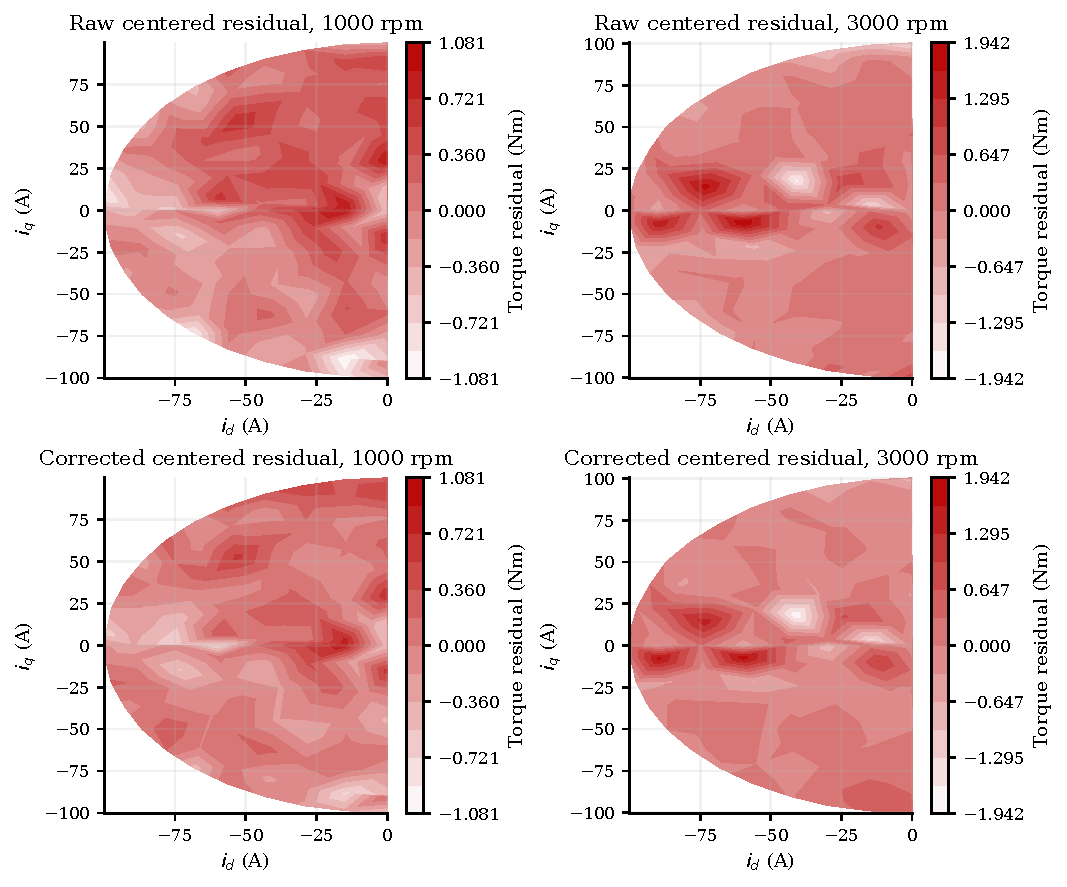
\includegraphics[width=\textwidth]{figures/09_real_residual_surfaces.pdf}
 \caption{Measured-minus-theoretical residual after subtracting each surface's
 group mean. The correction reduces some spatial structure but does not make the
 two speed slices equivalent. Color bars retain torque units.}
 \label{fig:real-residual-surfaces}
\end{figure}

\begin{figure}[htbp]
 \centering
 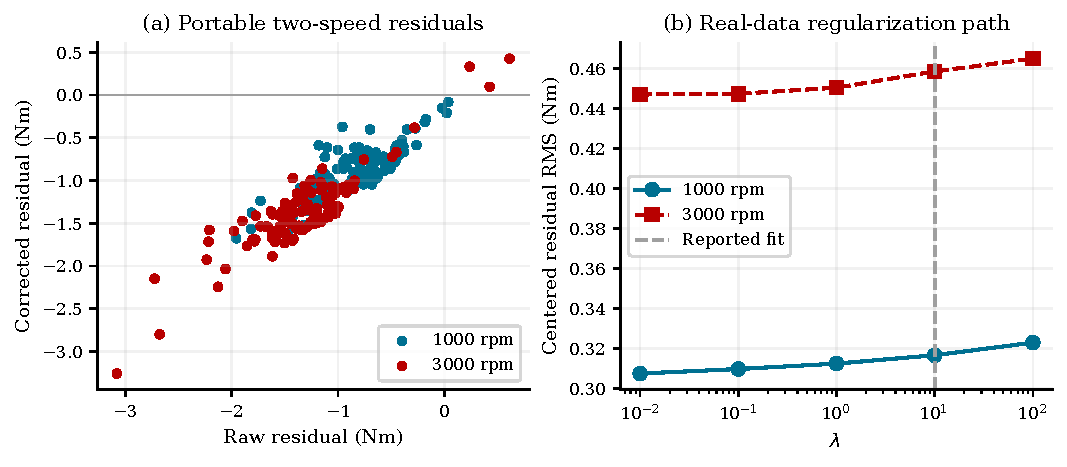
\includegraphics[width=\textwidth]{figures/10_real_regularization.pdf}
 \caption{Standalone two-speed summary. Left: raw and corrected residuals still
 include different nonzero offsets. Right: centered residual spread versus the
 declared regularization weight; no unknown real-flux RMSE is used for tuning.}
 \label{fig:real-regularization}
\end{figure}

\subsection{The decisive multi-speed transfer check}
A correction fitted only at 1000 rpm reduces its own centered residual but
increases the 3000-rpm spread; the converse fit likewise worsens 1000 rpm.
Consequently the available channel does not support interpreting either
single-speed fit as one speed-invariant magnetic correction. The joint fit is
a regularized descriptive compromise. Speed-dependent loss, voltage error,
sensor behavior or state mismatch remain plausible nuisance mechanisms.

Every operating point is written to \texttt{figures/data/real\_residuals.csv}
with raw and corrected flux, measured and theoretical torque, raw and corrected
residual, and the applied correction. The complete regularization path is a
second CSV; provenance, offsets, low-complexity diagnostics and transfer results
are stored in \texttt{numerics/real\_evaluation.json}.
